\section{Hierarchically Fused Fully Convolutional Network}
\label{Sec:HF-FCN}
In this section, we introduce a novel operation for feature fusion, named hierarchical fusion operation and apply it to the common networks, VGG16 Net and ResNet. The overview diagram in Fig.~\ref{fig:Fusion-Operation} shows where the fusion operations take effect and how they work. Different from other networks for semantic segmentation, we apply the fusion operation twice to integrate information gradually.
Our network consists of three parts. Part 1 is a bottom-up pathway which plays a role of features extractors at different levels.
In theory, arbitrary feature extraction network is applicable to the Part 1.
The second part is a process of feature fusion in the first stage, which fuses the feature maps generated from Part 1.
Besides, Part 3 is a second stage of feature fusion.
In Part 3, we take full advantage of the information extracted from the Part 2 by learning the connection weights between upsampled feature maps.

\begin{figure}
\vspace{-0.4cm}
\setlength{\abovecaptionskip}{-0cm}
\setlength{\belowcaptionskip}{-2cm} 
\centering
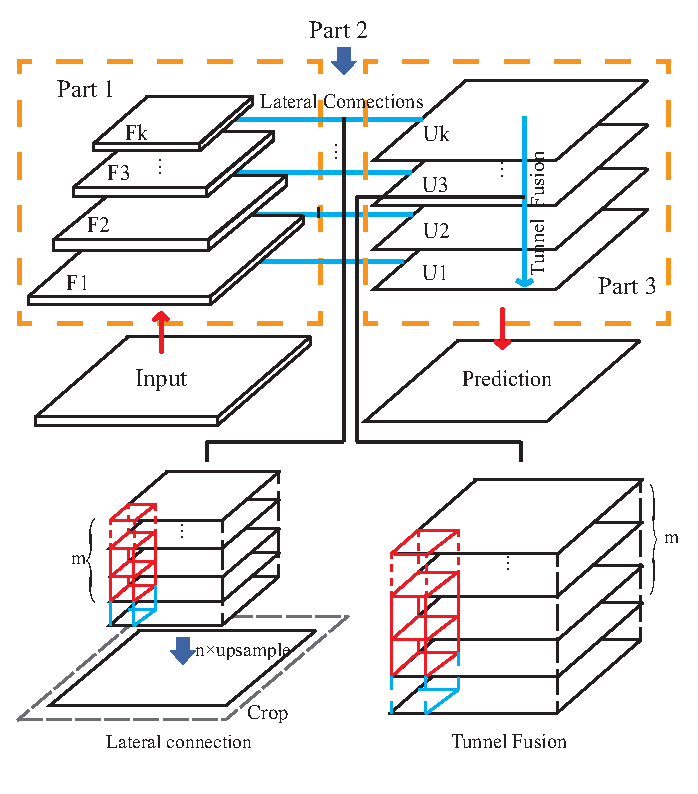
\includegraphics[width=8.5cm]{Figures/Fusion_Operation.eps}
\caption{The first line shows the overview of our network. The second row shows the details of two kinds of fusion operation. One is a case where the input is not equal to the output and the other is the input equal to the output. Fk means the feature maps come from the kth layer. m for number of feature maps. n said the n times of up sampling.}
\label{fig:Fusion-Operation}
\end{figure}
\cxj{Put overview here. Explain the main components of our methods.}
\subsection{Network Architecture}

\textbf{Part 1} The Part 1 is a bottom-up pathway, which generates the hierarchical feature maps from the network. With the increase of the field of perception, the extracted semantic information is gradually from the lower level to the high level. At the same time, the extracted information of image is from local to global. Each group of feature maps come from the same feature extractor contribute to the ${\left\{F_{k}\right\}}$ in Fig.~\ref{fig:Fusion-Operation}, where ${k:\Omega \to\left\{1,\ldots,K\right\}}$. And ${K}$ is group number of feature maps; for instance, ${K}$ is 13 for VGG16 Net that we consider each
convolution(conv) layer as a feature extractor. Specifically, for ResNets, we consider a ResBlock as a feature extractor that ${K}$ is 15.

\textbf{Part 2} The Part 2 which fuses the feature maps of each group extracted from Part 1 via a set of hierarchical fusion operations. Due to the feature maps learned from same group including similar types of information, we fuse them into one feature map, which contains richer information. The hierarchical fusion operation consists of three steps:
A ${1\times1}$ conv layer first, a deconvolutional (transposed convolution) layer second and crop operation third.
The Part 2 in Fig.~\ref{fig:Fusion-Operation} can be written as:
\begin{equation}
    \label{fusion_1}
    \ U_{k}=Crop(UpSample_n(Conv(\left\{F_{k}\right\})))
\end{equation}

where ${\left\{F_{k}\right\}}$ is a set of extracted feature maps from Part 1, ${k:\Omega \to\left\{1,\ldots,K\right\}}$.

The first step is a ${1\times1}$ conv operation among the channels of feature maps in the same group.
${Y = Conv(\left\{X\right\})}$ is defined as:
\begin{equation}
    \label{Conv}
    \ Y(i,j)=\sum_{m=1}^{M}w_{m}X_{m}(i,j)
\end{equation}

 where ${M}$ is the number of the feature maps in ${\left\{X\right\}}$. The ${w_{m}}$ is the weight of conv kernels, ${m:\Omega \to\left\{1,\ldots,M\right\}}$.

\begin{figure}
\vspace{-0.4cm}
\setlength{\abovecaptionskip}{-0cm}
\setlength{\belowcaptionskip}{-2cm} 
\centering
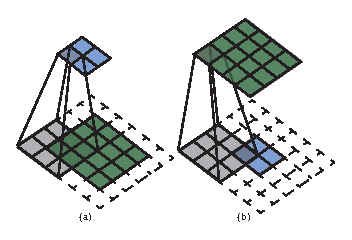
\includegraphics[width=8.5cm]{Figures/Conv_Deconv.eps}
\caption{A diagram of convolution and transposed convolution. The traditional convolution and transposed convolution are shown in the left and right column, respectively.
 The input of convolution is ${4\times4}$, the output is ${2\times2}$ and the kernel is ${3\times3}$. And the transposed convolution is the opposite.}
\label{fig:Deconv}
\end{figure}

If the input and output were to be unrolled into vectors form left to right, top to bottom, the convolution operation can be expressed as:
 \begin{equation}
    \label{Conv_matrix}
    \ y = Wx
\end{equation}

where ${x}$, ${y}$ are flattened vector of input and output. The ${W}$ is a sparse matrix whose non-zero elements are weights of kernels.
A diagram of conv operation is shown in Fig.~\ref{fig:Deconv}(a).
For Fig.~\ref{fig:Deconv}(a), ${x}$ is a 16-dimensional vector (the input ${X}$ is a ${4\times4}$ patch), ${y}$ is a 4-dimensional vector and ${W}$ is a matrix of ${4\times16}$.


The output of ${Conv\left\{F_{k}\right\}}$ are upsmapled by a transposed convolution which is written as ${Y = UpSample_n(X)}$, where ${n}$ means ${n}$ times up sampling. The ${n}$ in our network is determined by the size of input $X$ and output $Y$ that is equal to ${max\left\{\lceil Y.weight/X.weight\rceil , \lceil Y.height/X.height\rceil \right\}}$. Contrary to conv operation, the transposed conv is a process of transforming the features of low dimension to high dimension. It can be written in a inverse form of conv operation:
\begin{equation}
    \label{Conv_matrix}
    \ y = W_1^Tx
\end{equation}

where ${x}$, ${y}$ are flattened vector of input and output. The ${W_1^T}$ is a sparse matrix whose non-zeros elements are weights of deconvolutional kernels.
Fig.~\ref{fig:Deconv}(b) shows a diagram of transposed conv.
For Fig.~\ref{fig:Deconv}(b), ${x}$ is 4-dimensional vector (the input ${X}$ of transpose conv is a ${2\times2}$ patch), ${y}$ is a 16-dimensional vector and ${W_1^T}$ is a matrix of ${4\times16}$.

The ${W_1^T}$ of transposed conv layers of different groups are learned separately. It means that the transposed conv layers recovery semantic information from hierarchical feature maps.
The ${Crop(\left\{X \right\})}$ operation in Part 2 is just a center alignment crop which cuts the superfluous boundary of upsampled feature maps. The output ${\left\{U_k\right\}}$, ${k:\Omega \to\left\{1,\ldots,K\right\}}$ of Part 2 are in the same resolution of the network input.


\textbf{Part 3} Part 3 is the second fusion stage which aims to fuse the cropped feature maps from Part 2.
In this part, the fusion operation plays a role of feature weighting.
Using a ${1\times1}$ conv layer, a set of parameters ${w_k}$, ${k:\Omega \to\left\{1,\ldots,K\right\}}$ are learned to combine the hierarchical feature maps.
The expression of the Part 3 is as follows:
\begin{equation}
    \label{fature_selection}
    \ Y= Conv(\left\{U_k\right\})
\end{equation}
where ${Y}$ is output feature map. ${\left\{U_k\right\}}$ is input of Part 3 and output of Part 2.


In order to get a probability map of input, the output ${Y}$ of Part 3 is normalized by a sigmoid function:
\begin{equation}
    \label{Sigmoid}
    \ S(x) = \frac{1}{1+e^{-x}}
\end{equation}
After normalization, A probability map ${P}$ of rooftop is generated, each point in ${P}$ means the probability that pixel belongs to a rooftop.
If the pixel ${x(i,j)}$ belongs to a rooftop, the output ${P(i,j)\approx1}$.

\subsection{Network Training}

The ground truth $G$ in our dataset is labeled by 0 or 1 to indicate whether a pixel belongs to a roof or not. \cxj{only roof? or part of the building including facades?}
When a remote sensing image ${X}$ is inputted into the network, the output is a prediction probability map $P(X;W)$ of roof, where $W$ denotes all the parameters that learned by HF-FCN including first part, Part 2 and 3.
We use the sigmoid cross-entropy loss function to penalize each position on the prediction map formulated as:
\begin{small}
\begin{equation}
     \label{loss}
     \ L(W)\! =\! -\frac{1}{\vert I\vert}\sum_{i=1}^{\vert I \vert}\lbrack{\tilde{g}_i \log{P(X_{i};W)}\!+\!(1\!-\!\tilde{g}_i)\log(1\!-\!P(X_{i};W)}\rbrack
\end{equation}
\end{small}
where $\tilde{g}_i$ is label of $X_{i}$, ${i:\Omega \to\left\{1,\ldots,\vert I\vert\right\}}$, ${\vert I\vert}$ is the number of pixels in the input image ${X}$.
